\subsection{HMI} \label{sec:HMI}
In diesem Kapitel wird der Aufbau und die Funktionen des HMI erklärt. Das Kapitel behandelt die HMI Maske, die entwickelte Leiterplatte und eine Bedienungsanleitung für den Umgang mit dem Planting Robot.

\subsubsection{Aufbau}
Alle Bedieneinheiten des HMI sollten dem Operator einfach zugänglich auf einem Blech platziert sein. Um die Übersicht über die 11 Taster und 14 LEDs zu behalten wurde die HMI Maske (siehe Abb. \ref{fig:HMI_Maske}) gezeichnet. Die Maske wurde dabei auf eine transparente Folie aufgedruckt und auf das Aluminium Blech aufgeklebt.

\begin{figure}[H]
	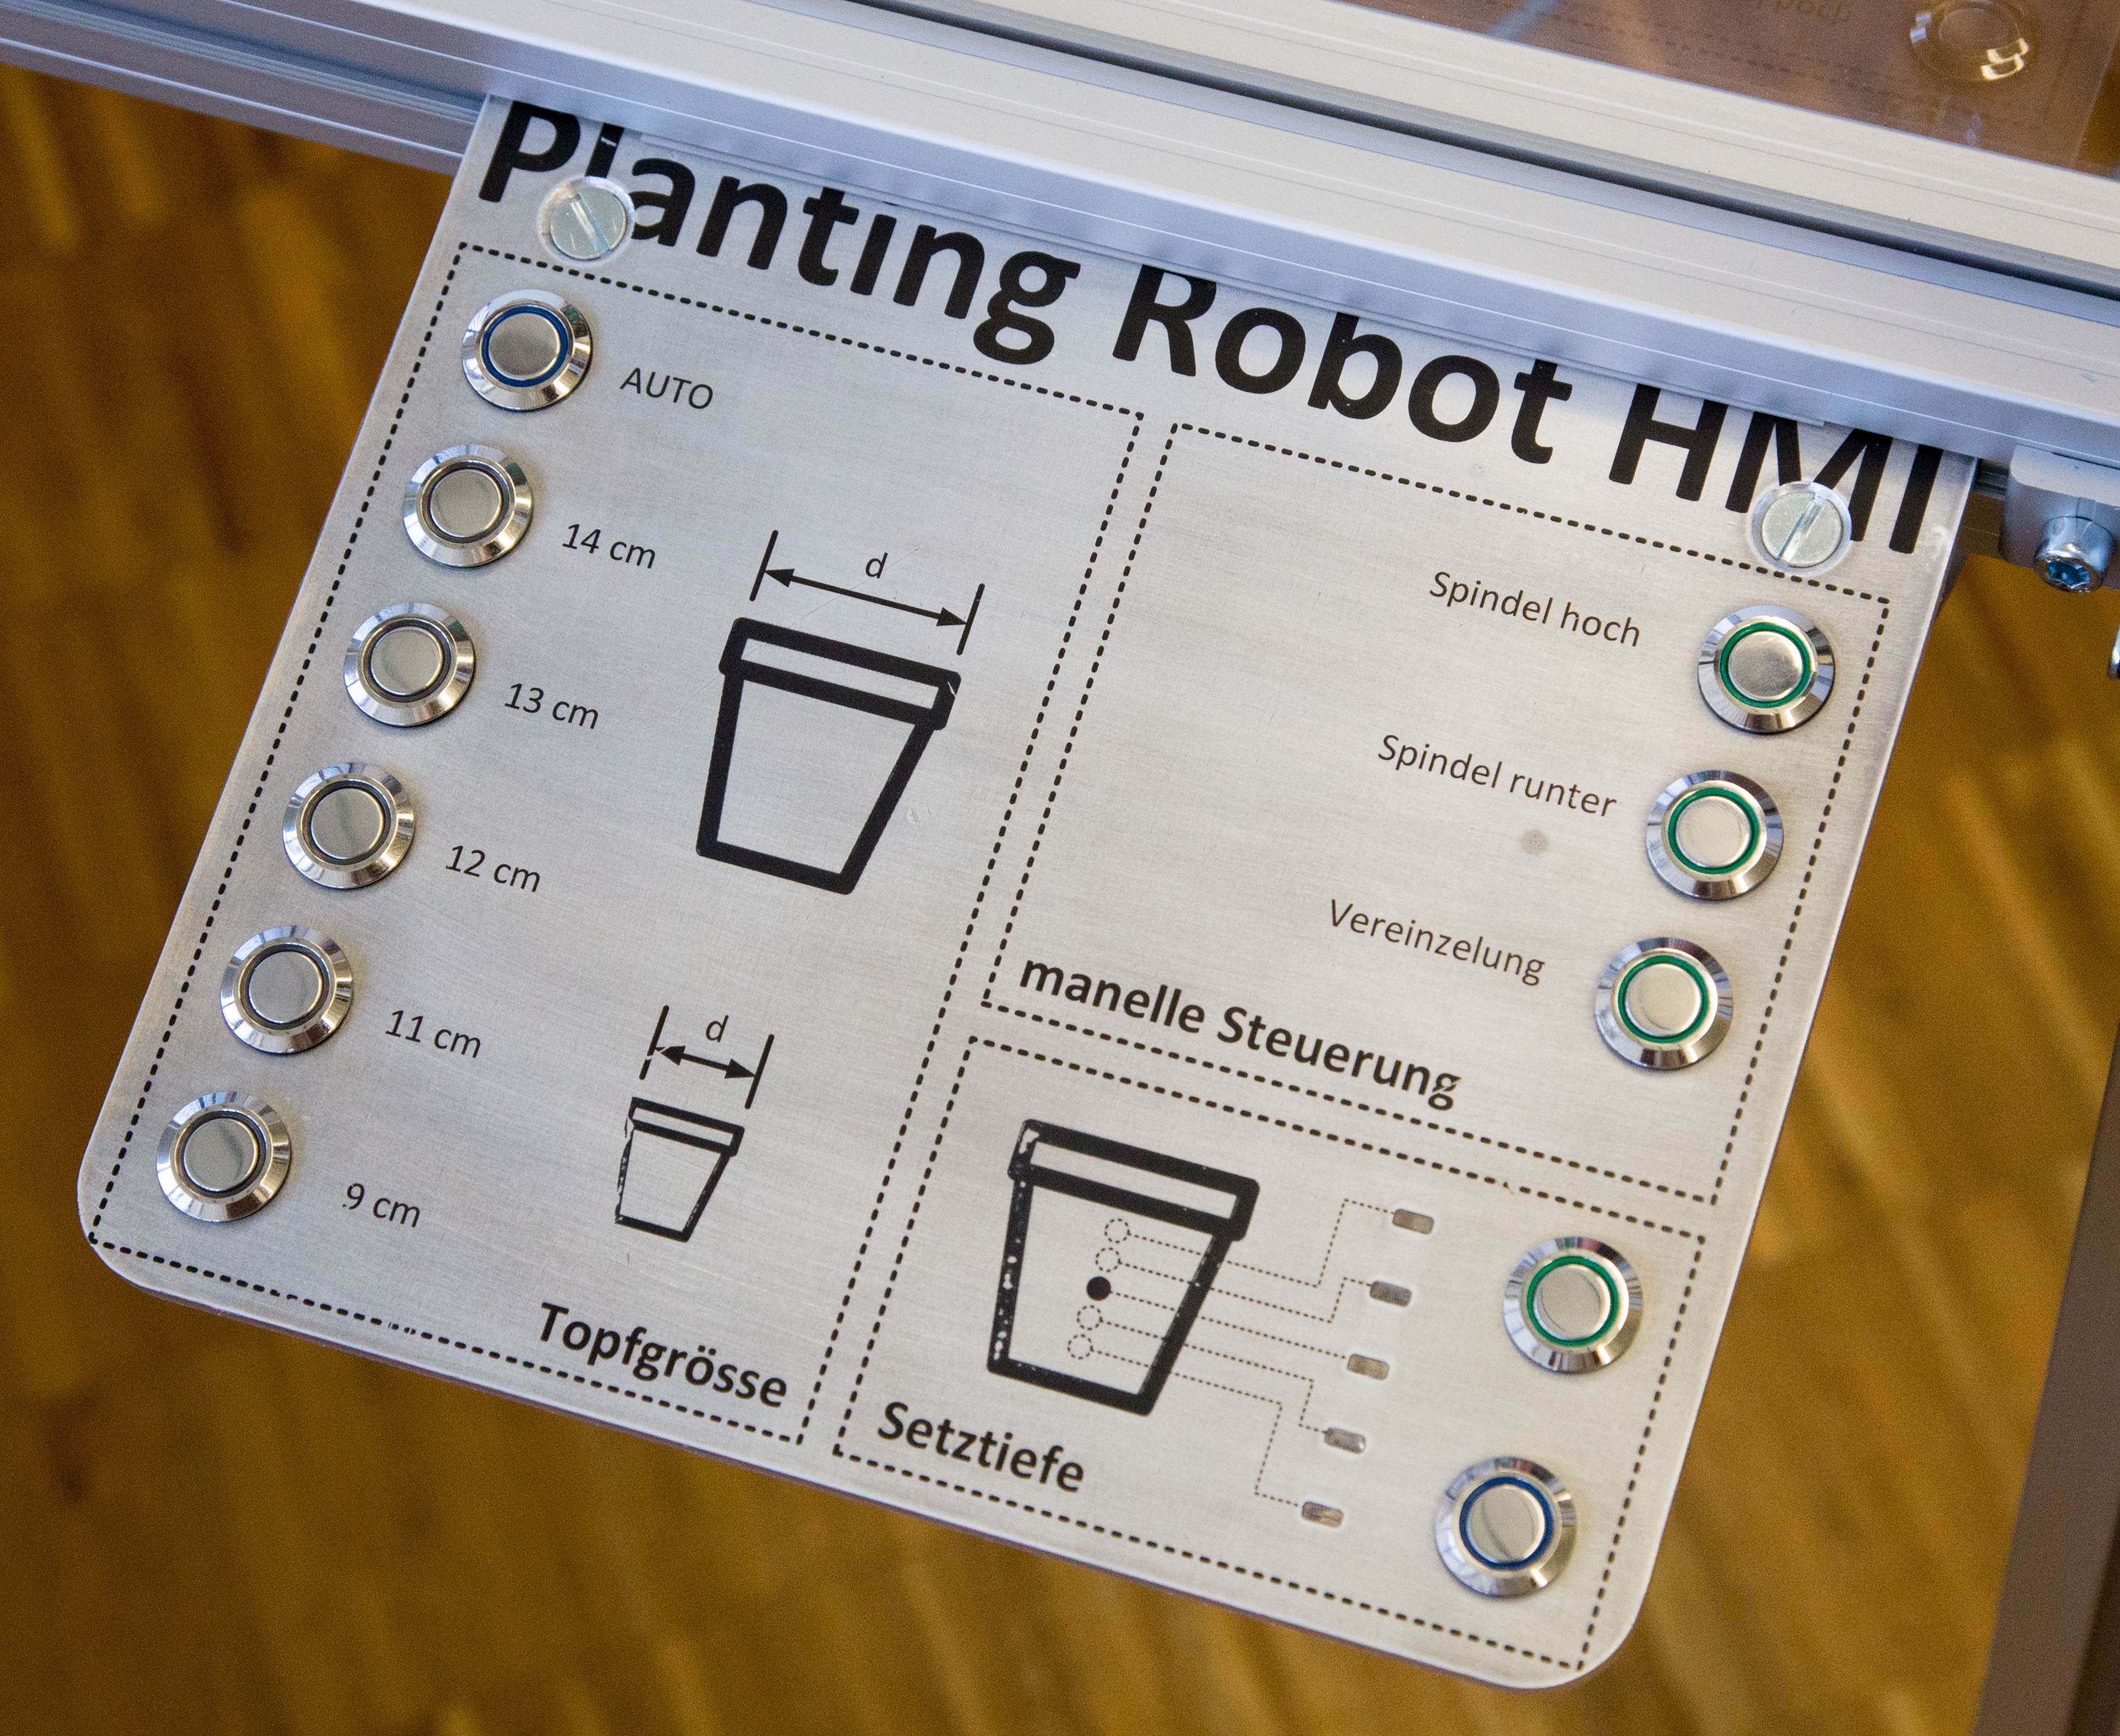
\includegraphics[draft=false,width=0.65\textwidth]{Illustrationen/6-Umsetzung/HMI_Foto.jpg}
	\caption{HMI Blech und Maske}
	\label{fig:HMI_Maske}
\end{figure}

Nebst den LEDs in den Drucktastern verfügt das HMI über 5 LEDs für die Anzeige der einstellbaren Setztiefe der NemaCaps. Diese LEDs sind auf dem HMI LED PCB bestückt und über light pipes durch das HMI Blech geführt. Light pipes ermöglichen das bündeln und führen von Licht. In dieser Anwendung werden sie verwendet um die LED Anzeige ästhetisch ansprechend auf dem HMI Blech zu integrieren.

\begin{figure}[H]
	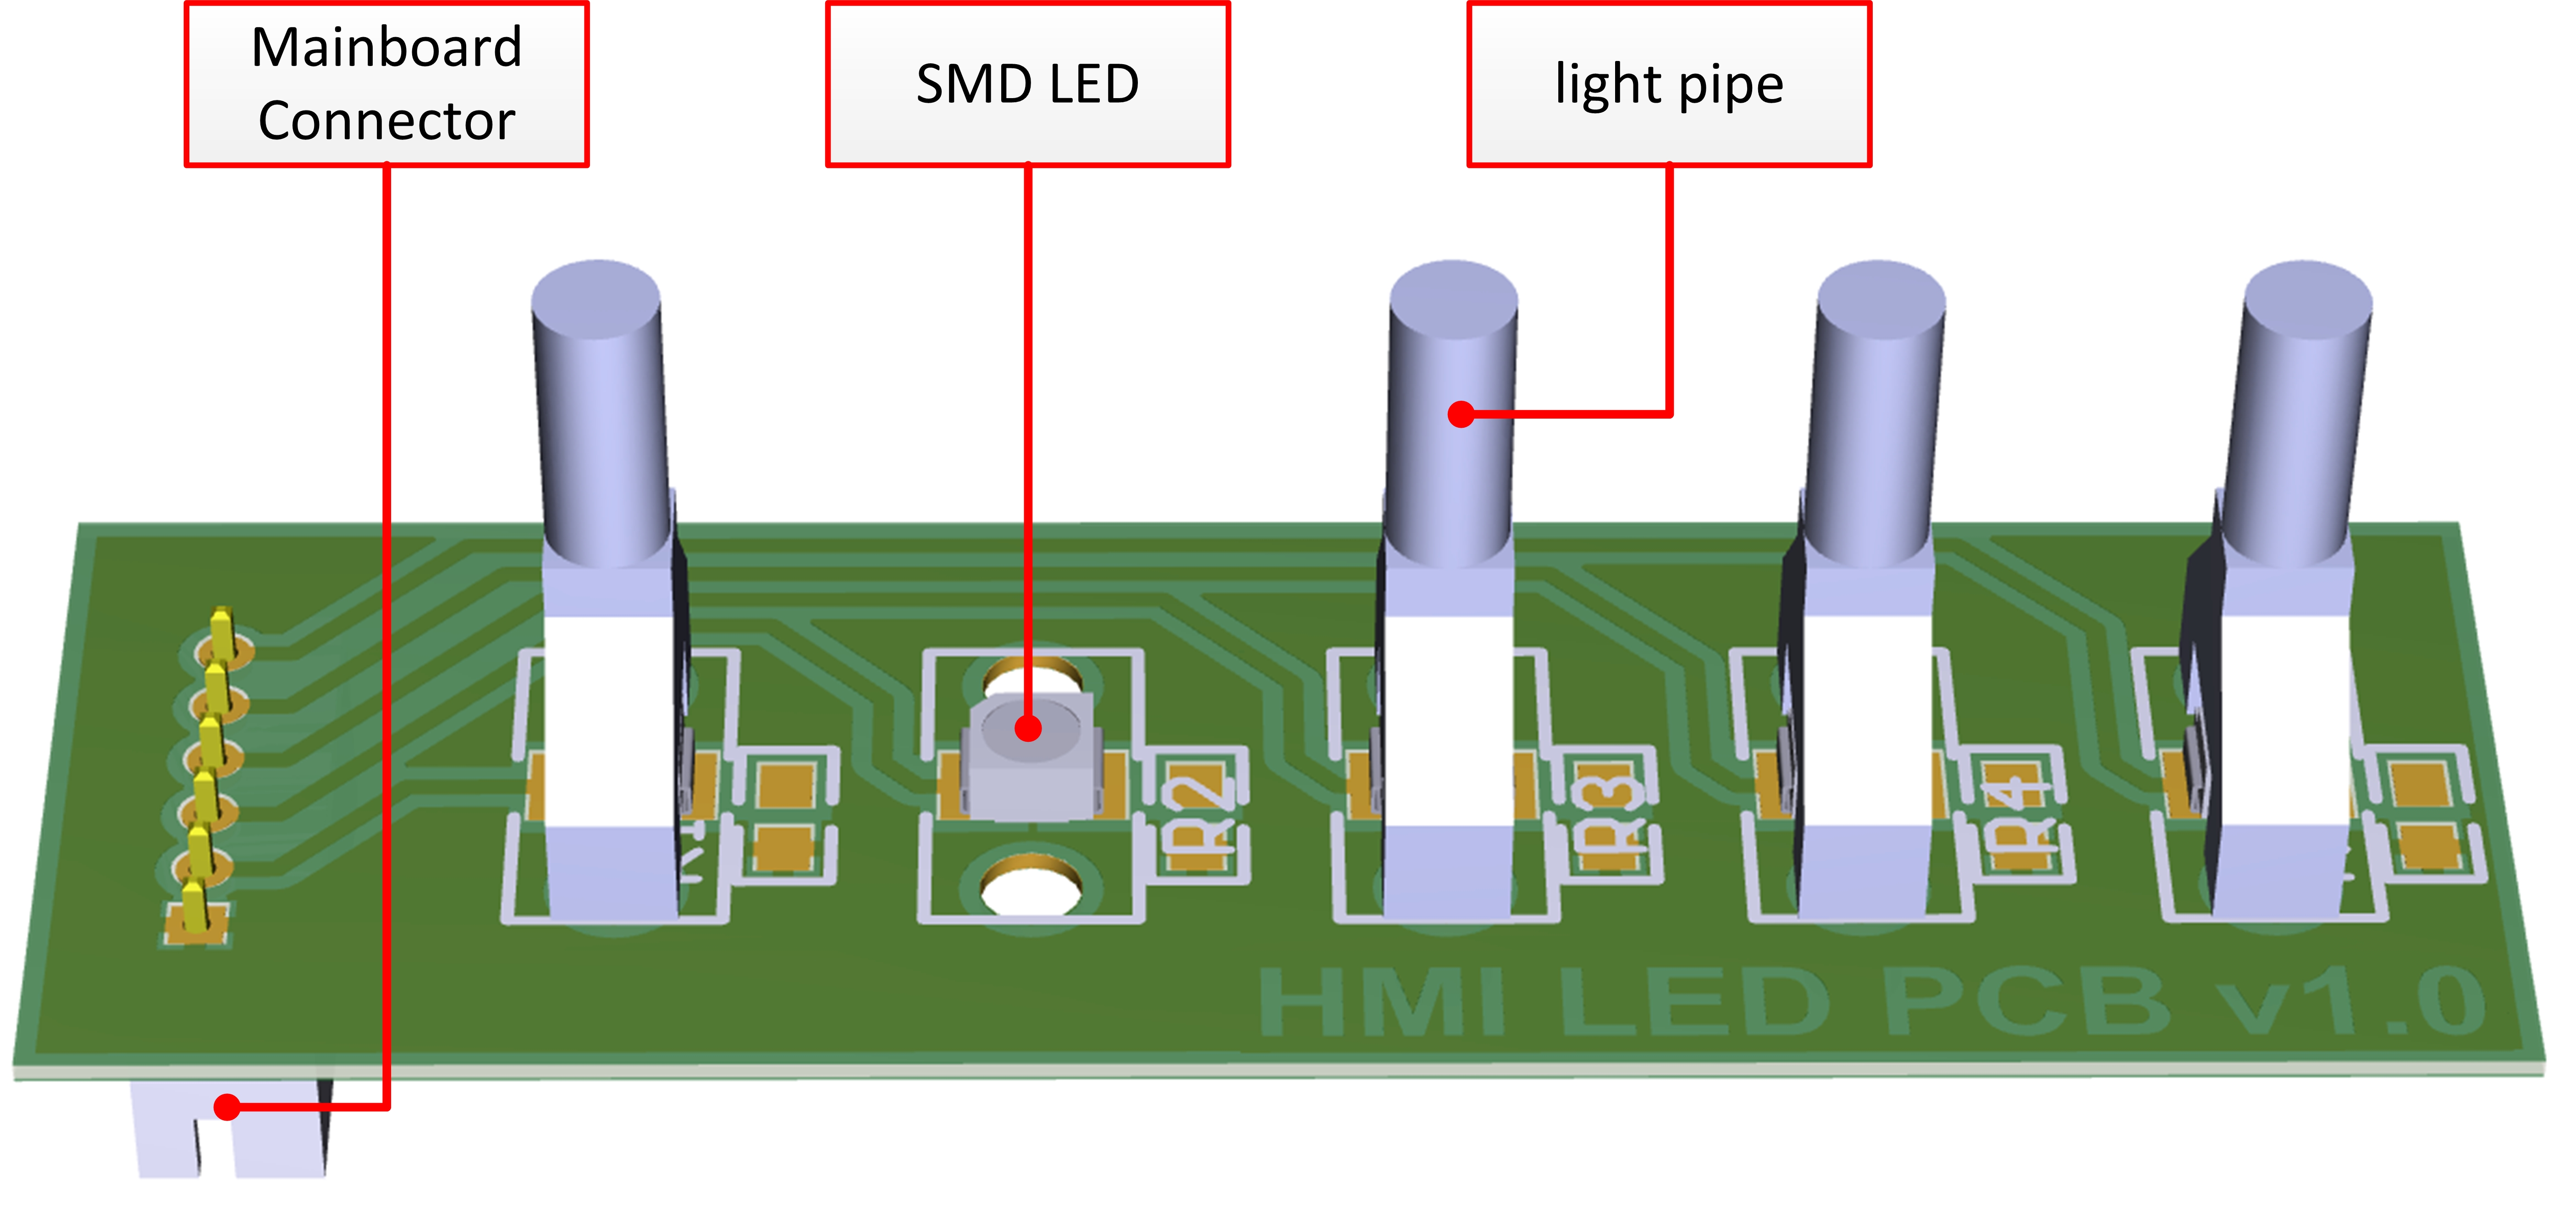
\includegraphics[draft=false,width=0.7\textwidth]{Illustrationen/6-Umsetzung/LED_PCB_3D.jpg}
	\caption{HMI LED PCB}
	\label{fig:LED_PCB_1}
\end{figure}

\subsubsection{Bedienungsanleitung}
Im folgenden Abschnitt wird die Bedienung des Planting Robots Schritt für Schritt erklärt. Achtung! Der Planting Robot ist ein Prototyp. Demnach kann es bei unsachgemässer Bedienung potenziell zu Fehlfunktionen kommen. Als grafische Hilfestellung zur Bedienungsanleitung dient eine State Übersicht der Software in Abb. \ref{fig:Bedienungsanleitung}.

\begin{figure}[H]
	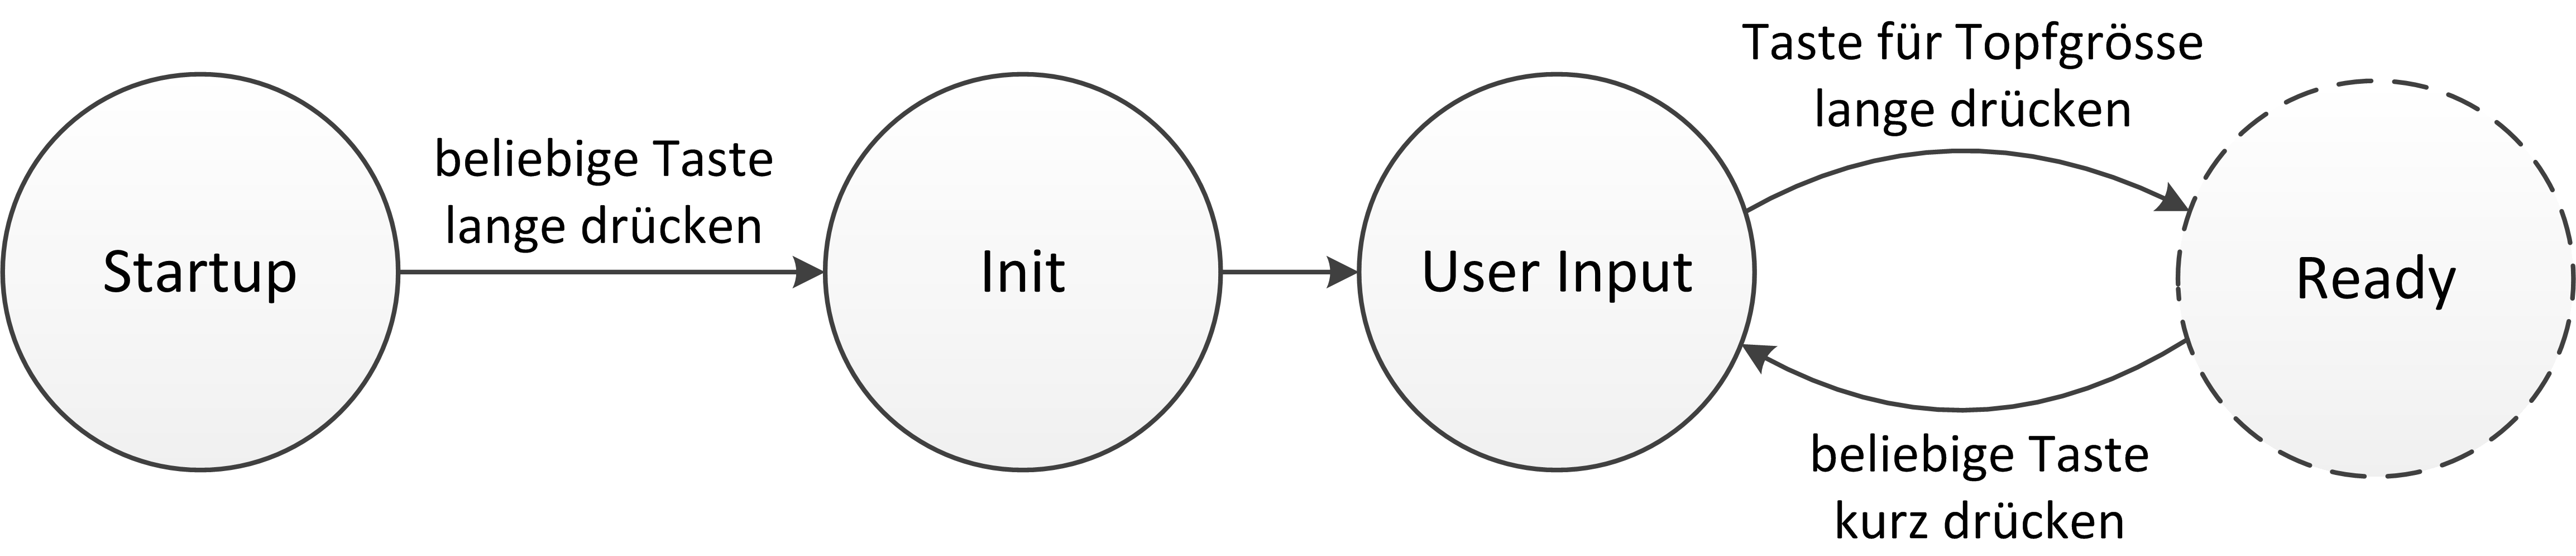
\includegraphics[draft=false,width=1\textwidth]{Illustrationen/6-Umsetzung/Bedienungsanleitung.png}
	\caption{Bedienungsanleitung, State Übersicht}
	\label{fig:Bedienungsanleitung}
\end{figure}

\begin{enumerate}
	\item Um den Planting Robot in Betrieb zu nehmen, muss der Einschalttaster auf der Rückseite des Maschinengestells gedrückt werden. Vergewissern Sie sich dabei, dass der Netzstecker eingesteckt und der Leitungsschutzschalter durchgeschaltet ist.
	\item Sofort nach drücken des Einschalttasters fangen die LEDs des HMIs an zu pulsieren. Der Planting Robot befindet sich im Startup State. In diesem State führt der Planting Robot keine seiner Funktionen aus. Durch einen langen Tastendruck (>0.5s) eines beliebigen Tasters, fängt der Planting Robot an seine Komponenten zu initialisieren. Dies wird durch das blinken der HMI Taster der entsprechenden Funktionen angezeigt. Die Initialphase dauert ca. 5... 10s.
	\item Nach Abschluss der Initialphase befindet sich die Software im User Input State. \textbf{Zu diesem Zeitpunkt muss sich die Setzeinheit an der obersten Ausgangsstellung befinden.} Ist dies nicht der Fall, muss der Planting Robot neu gestartet und die vorherigen Schritte wiederholt werden. Im User Input State können Einstellungen zu den Topfgrössen und der Setztiefe vorgenommen werden. Diese Funktionen werden im Unterkapitel $"$User Input$"$ erklärt. Durch langes drücken einer Topfgrössen Taste wird der Planting Robot in Betrieb gebracht.
	\item Die Software wechselt in den Ready State. Da die Topferkennung aus Zeitgründen nicht mehr implementiert wurde, führt der Planting Robot in diesem State ein Demo Programm aus und nicht wie in Kapitel \ref{sec:FSM} beschrieben den regulären Betriebsmodus. Das Demo Programm dient zu Vorführzwecken und kann durch einen beliebigen Tastendruck unterbrochen werden. Durch den Tastendruck wechselt die Software wieder zurück in den User $"$Input State$"$.
\end{enumerate}

\textbf{User Input}\\
Im $"$User Input$"$ State kann die Topfgrösse sowie die Setztiefe der Nemacaps konfiguriert werden. Um eine andere Topfgrösse einzustellen, muss auf dem HMI die entsprechende Grösse angewählt werden. Die Verstellmechanik führt den Befahl bei Tastendruck sofort aus und konfiguriert den Setzradius neu. Die Setztiefe wird auf dem HMI über 5 LEDs angezeigt. Dabei ist standardmässig die mittlere grüne LED aktiviert. Diese signalisiert eine mittlere Setztiefe. Durch drücken der beiden Taster rechts der LEDs kann die Setztiefe höher oder tiefer eingestellt werden. Diese Funktion ist in der Software der Setzeinheit noch nicht implementiert, die LEDs lassen sich zu Vorschauzwecken allerdings schon einstellen.\\
Eine weitere Funktion des $"$User Input$"$ States ist die manuelle Steuerung des Planting Robots. Über die Taster $"$Spindel hoch$"$ und $"$Spindel runter$"$ kann die Setzteinheit manuell hoch und runter bewegt werden. Die Taster müssen dafür länger als 0.5s gedrückt werden. Bei loslassen der Taster hält die Spindel wieder an. Durch Druck auf den Taster $"$Vereinzelung$"$ wird die Lochmaske der Vereinzelung um eine Position gedreht.